

\chapter{تصميم النظام}
يبيّن هذا الفصل منهجية العمل المتبعة خلال تنفيذ المشروع.
ويشرح النظام على مستوى عالي من التجريد وفق مخططات صندوقية.
كما يسرد الميزات التي استخراجها من النصوص.
ويسرد خوارزميات تعلم الآلة التي تم استخدامها.

\section{منهجية العمل}
نتعامل مع المسألة المطروحة ضمن المشروع على أنها مسألة تصنيف مقروئية نص مكتوب باللغة الانكليزية وفق عدّة مستويات.
فالغاية المرجوّة هي معرفة مستوى صعوبة نص معيّن وإلى أي مستوى ينتمي.
سؤال قد يتم طرحه هنا وهو: ما هو عدد المستويات وما هو التفاوت ومعيار المقارنة بينها؟
الإجابة هي أن عدد المستويات والفروقات بينها يتم تحديده ضمن المعطيات التي ستُستخدم لتدريب المصّنف.
فقد تكون هذه المعطيات مفصولة إلى أي عدد من المستويات.
ولكن وجِبَ أن يكون معيار المقارنة بين هذه المستويات هو مقروئية النصوص وذلك لكي يحقق التطبيق الناتج الهدف المرجو منه.

تبدأ أنظمة تعلم الآلة عادة بجمع المعطيات.
في حالتنا هذه، نريد جميع عدد كبير من النصوص المصنّفة بشكل مسبق وصحيح إلى مستوى صعوبة مقروئيتها.
لم نحتاج إلى القيام بهذه المرحلة ضمن المشروع بسبب توافر هكذا معطيات.
المرحلة التي تليها هي مرحلة استخراج الميزات.
إذ يتم التعبير عن المعطيات الخام بأشعة من الميزات يمكن لخوارزميات تعلم الآلة إجراء عمليات حسابية عليها.
وبعد استخراج الميزات، يتم اختيار خورازمية تعلم الآلة المناسبة وضبط برامتراتها 
لتدريبها على جزء من هذه المعطيات (معطيات التدريب) واختبارها على الجزء الآخر (معطيات الاختبار).
وذلك لتقييم مستوى أدائها ومعرفة الجدوى من استخدامها.

أخيراً بعد إجراء عملية التدريب والحصول على مُصنّف جاهز للاستخدام،
نقوم لأجل نص جديد باستخراج ميزاته واستخدام المصنّف للحصول على مستوى مقروئية هذا النص.


\section{المخططات الصندوقية للنطام}
كما رأينا في الفقرة السابقة، توجد عدّة مراحل لتنجيز النظام بشكل كامل.
ودون الخوض في كثير من التفاصيل، سنعتبر أنه توجد مرحلتان أساسيتان لتنجيز المشروع.
الأولى هي للحصول على مصنّف جاهز للاستخدام.
الثانية هي استخدام هذا المصنّف.

يبيّن الشكل~\ref{fig:sys:diag} المخطط الصندوقي للنظام الذي تم تنجيزه للحصول على المصنف وتقييم أدائه.
بينما يبيّن الشكل~\ref{fig:sys:use} المخطط الصندوقي لاستخدام هذا المصنف.
 \begin{figure}[htb] 
	\centering
	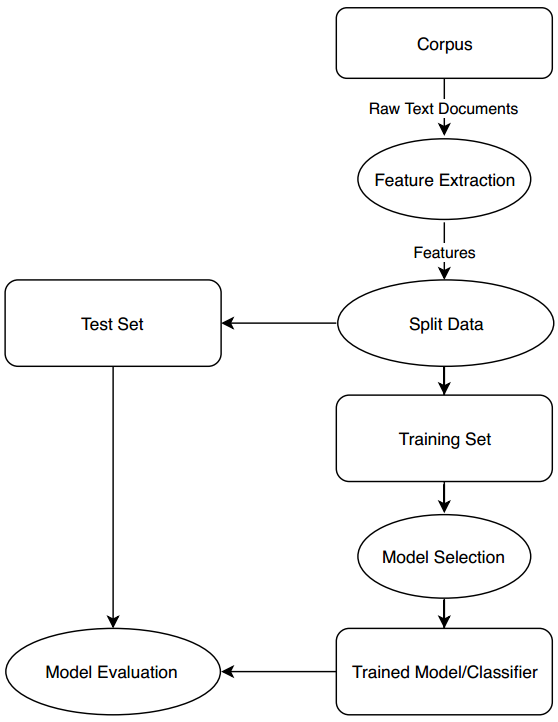
\includegraphics[width=0.65\linewidth]{images/sys_diag.png}
	\caption{%
		المخطط الصندوقي للحصول على المصنّف وتقييم أدائه.
	}
	\label{fig:sys:diag}
\end{figure}

 \begin{figure}[htb] 
	\centering
	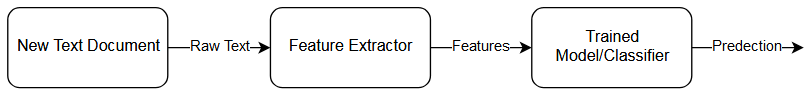
\includegraphics[width=0.9\linewidth]{images/sys_use.png}
	\caption{%
		المخطط الصندوقي لاستخدام المصنّف.
	}
	\label{fig:sys:use}
\end{figure}

\afterpage{\clearpage}

\section{المعطيات المستخدمة}
\label{sec:sys:datasets}
تبّين هذه الفقرة المعطيات المستخدمة ضمن المشروع وخصائصها.


\subsection{\eng{One Stop English Corpus (OSE)}}
يعود الفضل في تجميع هذه المعطيات إلى~\cite{vajjala2018}.
تم تجميع هذه المعطيات من الموقع
\url{http://www.onestopenglish.com}
في الفترة ما بين
$2013-2016$%
. وهو موقع تعليمي بأكثر من $700,000$ مستخدم  من $100$ دولة.

أحد ميزات هذا الموقع هو وجود درس تعليمي أسبوعي له طابع إخباري يحوي مقالات من الصحيفة البريطانية \eng{The Guardian}.
إذ تتم إعادة صياغة مقالات هذه الصحيفة من قبل المدرسين لتناسب ثلاثة مستويات من الطلاب
(مبتدأ \eng{elementary}، متوسط \eng{intermediate}، متقدم \eng{advanced}).
أي أنه تتم إعادة صياغة محتوى الصحيفة الأصلي إلى ثلاث نسخ متدرجة الصعوبة من حيث مقروئيتها مع المحافظة على أكبر قدر من فحوى المحتوى الأصلي.
يبيّن الجدول~\ref{tbl:corpus:ose} عيّنة من هذه المعطيات.

تُبيّن لنا طريقة جمع هذه المعطيات أهميتها بالنسبة للمشروع.
إذ إن معيار المقارنة بين هذه المستويات هو مقروئية النصوص من ناحية تعقيد تراكيب الجمل أو بساطتها وذلك لنصوص لها نفس الفحوى.
وإجراء الاختبارات عليها سيوضح الجدوى من استخدام هذا النظام في تحليل مقروئية النصوص من ناحية الصياغة.

\begin{table}[htb]
	\centering
	{
		\setlength{\tabcolsep}{0.5em} % for the horizontal padding
		\renewcommand{\arraystretch}{1.4}% for the vertical padding
		\selectlanguage{english}
		
		\begin{tabular}{|>{\arraybackslash}p{0.2\textwidth}|>{\arraybackslash}p{0.7\textwidth}|}
			\hline
			\textbf{Reading Level} &
			\textbf{Sample Text} \\
			\hline 
			Elementary &
			To tourists, Amsterdam still seems very liberal. Recently the city’s Mayor told
			them that the coffee shops that sell marijuana would stay open, although there
			is a new national law to stop drug tourism. But the Dutch capital has a plan
			to send antisocial neighbours to scum villages made from shipping containers,
			and so maybe now people wont think it is a liberal city any more. \\
			\hline 
			Intermediate &
			To tourists, Amsterdam still seems very liberal. Recently the city’s Mayor assured them that the city’s marijuana-selling coffee shops would stay open despite a new national law to prevent drug tourism. But the Dutch capitals plans
			to send nuisance neighbours to scum villages made from shipping containers
			may damage its reputation for tolerance. \\
			\hline 
			Advanced &
			Amsterdam still looks liberal to tourists, who were recently assured by the
			Labour Mayor that the city’s marijuana-selling coffee shops would stay open
			despite a new national law tackling drug tourism. But the Dutch capital may
			lose its reputation for tolerance over plans to dispatch nuisance neighbours to
			scum villages made from shipping containers. \\
			\hline 
		\end{tabular}
	}
	\caption{%
		عيّنة من جمل الـ \eng{OSE} المصنفة إلى ثلاثة مستويات.
	}
	\label{tbl:corpus:ose}
\end{table}

تتألف هذه المعطيات من $567$ نص موزعين بالتساوي إلى المستويات الثلاثة،
أي يوجد $189$ نص في كل مستوى.
ويبّن الجدول~\ref{tbl:corpus:ose_stat} بعض الإحصائيات الوصفية لنصوص هذه المعطيات.
وهي متوسط طول النص، والانحراف المعياري لطول النص وذلك للمستويات الثلاثة كلاً على حدا.
وإن الواحدة المستخدمة لطول النص هي الكلمة.
نلاحظ (كما هو متوقع) أن الطول الوسطي للنصوص يتزايد مع تزايد المستوى.
وأن الانحراف المعياري لطول النصوص كبير مما يجعل طول النص معيار غير كافي لتحديد صعوبته.

\begin{table}[htb]
	\centering
	{
		\setlength{\tabcolsep}{0.5em} % for the horizontal padding
		\renewcommand{\arraystretch}{1.4}% for the vertical padding
		\selectlanguage{english}
		
		\begin{tabular}{|c|c|c|}
			\hline
			
			\textbf{Reading Level} &
			\textbf{Avg. Num. Words} &
			\textbf{Std. Dev.}\\
			\hline 
			
			Elementary &
			533.17 &
			103.79 \\
			\hline
			
			Intermediate &
			676.59 &
			117.15 \\
			\hline
			
			Advanced &
			820.49 &
			162.52 \\
			\hline
			
		\end{tabular}
	}
	\caption{%
		إحصائيات وصفية لنصوص الـ \eng{OSE}.
	}
	\label{tbl:corpus:ose_stat}
\end{table}

هذه النصوص متاحة على الرابط
\url{https://github.com/nishkalavallabhi/OneStopEnglishCorpus}
ويجب التنويه إلى أن هذه المعطيات لم تسخدم كما هي، بل تم إجراء تنضيف شبه يدوي عليها.
حيث أنه وُجِدَت مجموعة من المحارف الغريبة التي تم استبدالها بمحارف مناسبة بحسب سياق ورودها ضمن النصوص.
فقد سبب بعض هذه المحارف مشاكل في قراءة النص أو استخدام مكتبات معالجة اللغات الطبيعية.
بالإضافة إلى كونها تشكل تشويش في المعطيات.
فيمكن اعتبار أن أحد منجزات هذا المشروع هو تنظيف معطيات الـ \eng{OSE} بالكامل وبإشراف شبه يدوي.

\section{الميزات المستخدمة}
\label{sec:sys:features}



\section{الخوارزميات المستخدمة}



